\vspace{.25cm}
\begin{figure}[ht!]
\centering
	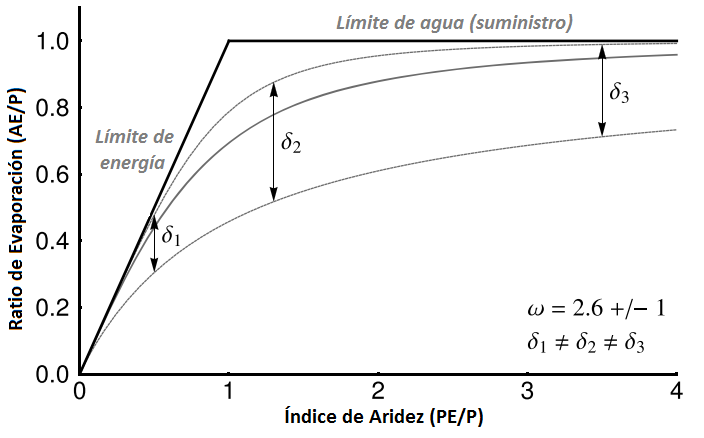
\includegraphics[scale=0.7]{Images/Greve2015_original_budyko.png}
	\caption{Tradicional curva de Budyko (correspondiente a un $\omega = 2.6$ \citep{Fu1981,Zhang2004}, línea gris) ubicando por $\omega = 2.6 \pm 1$ (líneas delgadas). La distancia Euclidiana ($\delta$) entre las curvas es diferente para cada valor de $PE/P$.}
	{\raggedright FUENTE: \citet{Greve2015}. \par}
	\label{fig:Greve01}
\end{figure}
